\section{Protein synthesis}

Lastly, we turn our attention to the process of translation. So far our
estimates have led to protein copy numbers that are consistent with the
proteomic data, or even in excess of what might be needed for each task under
limiting growth conditions. Even in our example of \textit{E. coli} grown under
different carbohydrate sources (\FIG{carbon_tport}(B)), cells can utilize
alternative carbon sources by inducing the expression of additional membrane
transporters and enzymes. Optimal resource allocation and the role of ribosomal
proteins have been an area of intense quantitative study over the last decade by
Hwa and others \citep{scott2010, hui2015}. From the perspective of limiting
growth, our earlier estimate of rRNA highlighted the necessity for multiple
copies of rRNA genes in order to make enough rRNA, suggesting the possibility
that synthesis of ribosomes might be rate limiting. While the transcriptional
demand for  the ribosomal proteins is substantially lower than rRNA genes, since
many proteins can be translated from relatively fewer mRNA, other ribosomal
proteins like the translation elongation factor EF-Tu also present a substantial
burden. For EF-Tu  in particular, it is the most highly expressed protein in
\textit{E. coli} and  is expressed by multiple genes on the chromosome, tufA and
tufB.

% Experimentally,
% consecutive deletion of rRNA operons showed a significant reduction in growth
% rate in rich media when cells had only 3 or less \citep{levin2017}.

% Separately, it has been found that gross
% overexpression of a protein can dramatically lower growth rate due to the
% altered allocation of resources \citep{basan2015}.

We begin by first estimating the number of tRNA synthetases and ribosomes
required for  a doubling time of 5000 seconds.  \textit{E. coli} has roughly 3 x
10$^6$ proteins per cell, which for an average protein of 300 aa, amounts to the formation
of $\approx$ 10$^9$ peptide bonds. This also corresponds to the
number of amino-acyl tRNA that are used by ribosomes, with the pool of tRNA continuously
recharging new amino acids by tRNA synthetases. At a rate of charging of
about 20 amino-acyl tRNA per second (BNID: 105279, \cite{milo2010}), we find
that cells have more than sufficient tRNA synthetases to meet the demand of
ribosomes during  protein synthesis (\FIG{protein_synthesis}(A)).
If we consider an elongation rate of $\approx$ 15 peptide bonds per second
(BNID: 114271, \cite{milo2010, dai2016}), the formation of $\approx$ 10$^9$
peptide bonds would require 1.5 x 10$^4$ ribosomes at a growth rate of 0.5
hr$^{-1}$. This is indeed consistent with the experimental data shown in
\FIG{protein_synthesis}(B).

[NB: How about moving this estimates paragraph and associated \FIG{protein_synthesis} to SI after all?]

\begin{figure}
    \begin{fullwidth}
    \centering{
        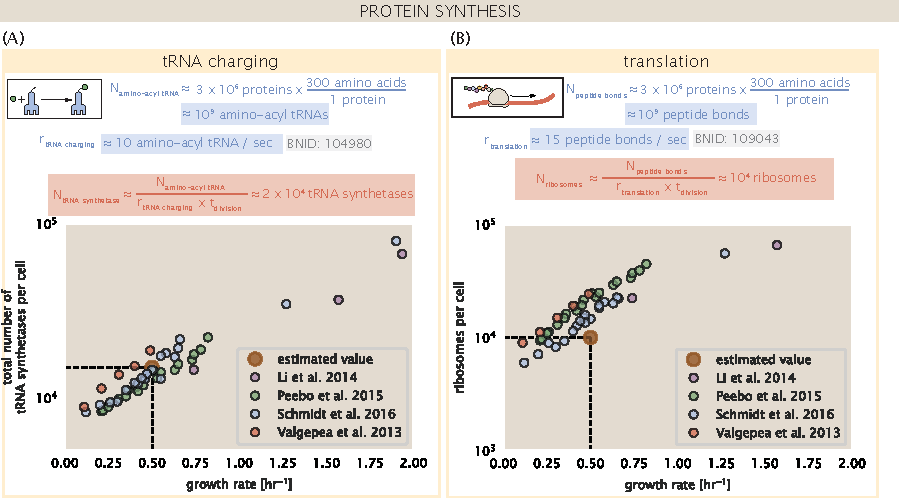
\includegraphics{main_figs/protein_synthesis.pdf}
        \caption{\textbf{Estimation of the required tRNA synthetases and
        ribosomes.} (A) Estimation for the
        number of tRNA synthetases that will supply the required amino acid
        demand. The sum of all tRNA synthetases copy numbers are plotted as a
        function of growth rate ([ArgS], [CysS], [GlnS], [GltX], [IleS], [LeuS],
        [ValS], [AlaS]$_2$, [AsnS]$_2$, [AspS]$_2$, [TyrS]$_2$, [TrpS]$_2$,
        [ThrS]$_2$, [SerS]$_2$, [ProS]$_2$, [PheS]$_2$[PheT]$_2$, [MetG]$_2$,
        [lysS]$_2$, [HisS]$_2$, [GlyS]$_2$[GlyQ]$_2$). (B) Estimation for the
        number of ribosomes required to synthesize all proteins in the cell. The
        average abundance of ribosomes is plotted as a function of growth rate.
        Our estimated values are shown for a growth rate of 0.5 hr$^{-1}$.}
    \label{fig:protein_synthesis}
    }
    \end{fullwidth}
\end{figure}

We can begin to gain some intuition into how translation might limit growth by
noting that the total number of peptide bonds generated as the cell doubles,
$N_{aa}$, which we used in our calculation above, will be given by, $\tau \cdot
r_t \cdot R$. Here, $\tau$ refers to the doubling time of the cell under
steady-state growth, $r_t$ is the maximum translation elongation rate, and $R$
is the average number of ribosomes per cell. With the growth rate related to the
cell doubling time by $\lambda = ln(2)/\tau$, we can write the
translation-limited growth rate as,

\begin{equation}
\lambda_{\textrm{translation-limited}} = \frac{ln(2) \cdot r_t \cdot R}{N_{aa}}.
\end{equation}
Alternatively, since $N_{aa}$ is related to the total protein mass through the
molecular weight of each protein, we can also consider the growth rate in terms
of ribosomal mass fraction. By making the approximation that an average amino
acid has a molecular weight of 110 Da (see \FIG{translation_1}(A)), we can
rewrite the growth rate as,

\begin{equation}
\lambda_{\textrm{translation-limited}} \approx \frac{ln(2) \cdot r_t}{L_R}  \Phi_R,
\label{eq:translation_limit_growth_rate}
\end{equation}
where $L_R$ is the total length in amino acids that make up a ribosome, and
$\Phi_R$ is the ribosomal mass fraction. This is plotted as a function of
ribosomal fraction $\Phi_R$ in \FIG{translation_1}(A), where we take $L_R
\approx $7459 aa, corresponding to the length in amino acids for all ribosomal
subunits of the 50S and 30S complex. This formulation assumes that the cell can
transcribe the required amount of rRNA, which appears reasonable for  \textit{E.
coli} under the  allowing us to consider the inherent limit on growth set by the
ribosome.

The growth rate defined by Equation \ref{eq:translation_limit_growth_rate}
reflects  mass-balance under steady-state growth and has long provided a
rationalization to the apparent linear increase in \textit{E. coli}'s ribosomal
content as a function of growth rate \citep{Goldberger1979, scott2010}. For our
purposes, there are several important consequences of this  trend. Perhaps the
first thing to notice is that there is a maximum growth rate at about $\lambda
\approx 6 hr^{-1}$, or doubling time of about 7 minutes (dashed line). This
growth rate can be viewed as an inherent maximum growth rate due to the need for
the cell to double the cell's entire ribosomal mass. Interestingly, this limit
is independent of the absolute number of ribosomes, but rather is simply given
by time to translate an entire ribosome, $L_R/ r_t$. As shown in
\FIG{translation_1}(B), we can reconcile this with the observation that in order
to double the average number of ribosomes, each ribosome must produce a second
ribosome. This is a process that cannot be parallelized.

For reasonable values of $\Phi_R$, between about 0.1 - 0.3 \citep{scott2010},
the maximum growth rate is in line with experimentally reported growth rates
around 0.5 - 2 $hr^{-1}$. Here we are implicitly assuming that translation
proceeds randomly, without preference between ribosomal or non-ribosomal mRNA,
which appears reasonable. Importantly, in order for a cell to scale this growth
limit set by $\Phi_R$, cells \textit{must} increase their ribosomal abundance.
This can be achieved by either synthesizing more ribosomes or reducing the
fraction of non-ribosomal proteins. Reduction of non-ribosomal proteins is not
straight forward since, as we have found throughout our estimates, doubling a
cell requires a substantial number of other enzymes and transporters. Increasing
the absolute ribosomal abundance is constrained by production of rRNA.

\begin{figure}
  \begin{fullwidth}
        \centering{
            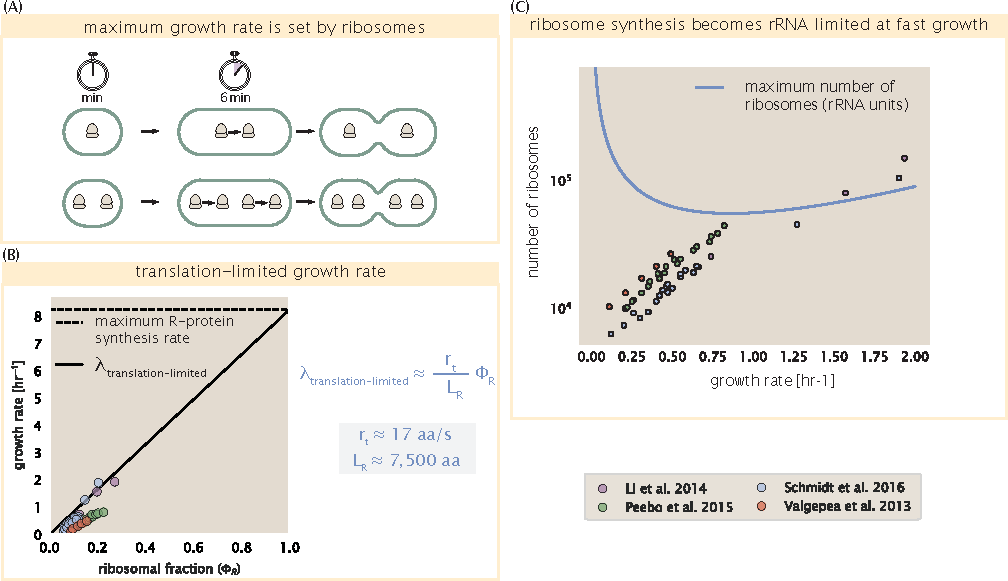
\includegraphics{main_figs/fig7_ribosome_growth_limit_2.pdf}
            \caption{\textbf{Translation-limited growth rate.} (A) Here we
            consider the translation-limited growth as a function of ribosomal
            fraction. By mass balance, the time required to double the entire
            proteome ($N_{aa}$ /$r_t \cdot $) sets the translation-limited
            growth rate, $\lambda_{\textrm{translation-limited}}$. Here $N_{aa}$
            is effectively the number of peptide bonds that must be translated,
            $r_t$ is the translation elongation rate, and $R$ is the number of
            ribosomes. This can also be re-written in terms of the ribosomal
            mass fraction $\Phi_R = m_R$ / $m_{\textrm{protein}}$, where $m_R$
            is the total ribosomal mass and $m_{\textrm{protein}}$ is the mass
            of all proteins in the cell. $L_R$ refers to the summed length of
            the ribosome in amino acids.
            $\lambda_{\textrm{translation-limited}}$ is ploted as a function of
            $\Phi_R$ (solid line). (B) The dashed line in part (A) identifies a
            maximum growth rate that is set by the ribosome. Specifically, this
            growth rate corresponds to the time required to  translation an
            entire ribosome, $L_R/ r_t$ . This is a result that is independent
            of the number of ribosomes in the cell as shown schematically here.
            (C) Schematic showing translation-specific requirements for maintenance
            of steady-state growth. In a nutrient rich environment, amino acid supply $r_{aa}$ is sufficiently in
            excess of demand by ribosomes translating at their maximal rate. In poorer
            nutrient conditions, reduced amino acid supply $r_{aa}$ will decrease
            the rate of elongation. In a regime where $r_{aa}$ is less than $r_t \cdot R$,
            the number of actively translating ribosomes will need to be reduced in order
            to maintain steady-state growth.}
        \label{fig:translation_1}
        }
  \end{fullwidth}
\end{figure}

While it is common for bacteria to decrease their ribosomal abundance in poorer
nutrient conditions \cite{scott2010, liebermeister2014}, this does not decrease
to zero. From the perspective of a bacterium dealing with uncertain nutrient
conditions, there is likely a benefit for the cell to maintain some relative
fraction of ribosomes to support rapid growth as nutrient conditions improve.
However, if we consider a scenario where nutrient conditions become poorer and
poorer, there will be a regime where ribosomes are in excess of the nutrient
supply. If the cell is to maintain steady-state growth, it will need to
attenuate its translational activity since ribosomes would otherwise exhaust
their supply of amino acids and bring cell growth to a halt
(\FIG{translation_1}(C)). In the next section we will consider this more
specifically for \textit{E. coli}, which has been shown to maintain a relatively
high elongation rate even in stationary phase ($\approx$ 8 aa/s, \cite{dai2016})
where cell growth is minimal.

[NB: I'm considering moving this paragraph near the end of the next section].

% In addition,
% given their massive size at about 850 kDa, they may play an as-yet fully
% understood role as a crowding agent in cellular function \cite{delarue2018,
% solerbistue2020}.

\subsection{Multiple replication forks bias ribosome abundance.}

\textit{E. coli} cells grow by an adder mechanism, whereby cells add a constant
volume with each cell division \citep{taheriaraghi2015}. In conjunction with
this, additional rounds of DNA replication are triggered when cells reach a
critical volume per origin of replication (\FIG{translation_ecoli}(A)). This
leads to the classically-described exponential increase in cell size with growth
rate \cite{schaechter1958, si2017, si2019}. In the context of maximizing growth
rate, it is notable that the majority of ribosomal proteins and rRNA operons are
found closer to the DNA origin. Given the need to increase to total gene dosage
of rRNA operons at faster growth rates, this raises the possibility that the
observed size scaling and increase in chromosomal equivalents might simply be
a means for the cell to tune biosynthesis according to their
physiological state.

While an increase in transcription has been observed for genes near the origin
in rapidly growing \textit{E. coli}  \citep{scholz2019}, we were unaware of such
characterization at the proteomic level. In order to test whether there is a
relative increase in protein expression for genes closer to the origin, we
calculated a running boxcar average of protein copy number as a function of
each gene's transcriptional start site. While absolute protein copy numbers can vary
substantially across the chromosome, we indeed observe a bias in expression
under fast growth conditions (\FIG{translation_ecoli}(B), showing the result
using a 0.5 kb averaging window). The dramatic change in protein copy number
near the origin mainly reflects the increase in ribosomal protein expression.
This trend is in contrast to slower growth conditions where the average copy
number is more uniform across the length of the chromosome.

\begin{figure*}
    \begin{fullwidth}
    \centering{
        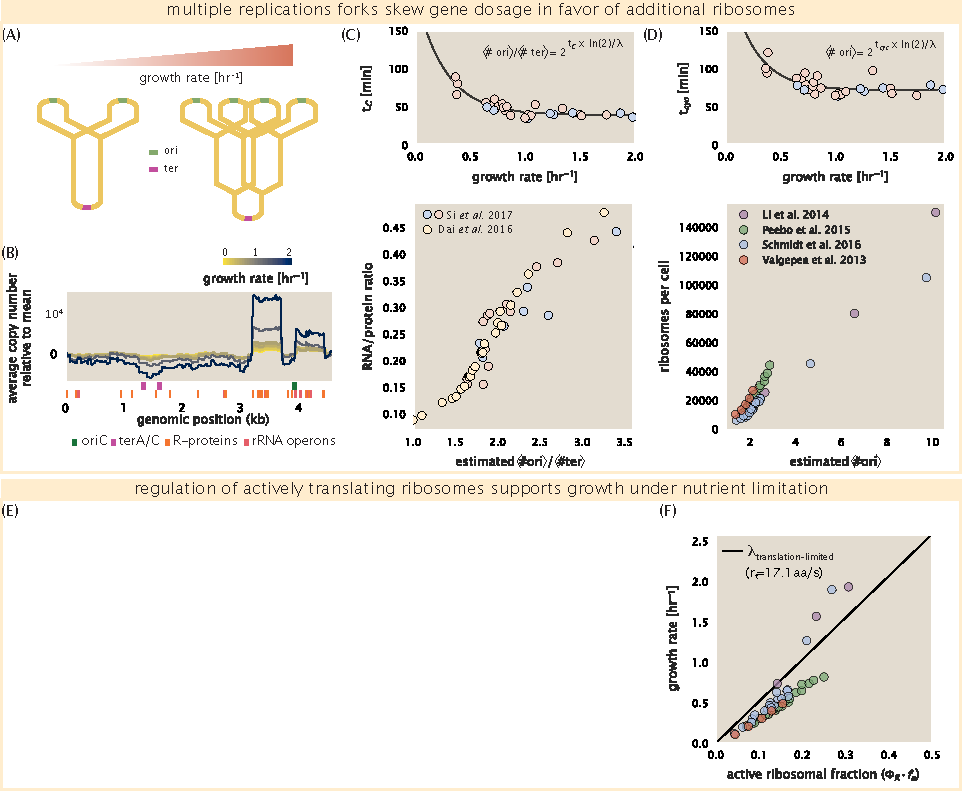
\includegraphics{main_figs/fig8_ribosome_growth_limit_ecoli_temp.pdf}
        \caption{\textbf{Multiple replication forks skew gene dosage and
        ribosomal content.} (A) Schematic shows the expected
        increase in replication forks (or number of ori regions) as \textit{E. coli} cells
        grow faster. (B) A running boxcar average of protein copy number is calculated for
        each each growth condition considered by
        Schmidt \textit{et al.}. A 0.5 kb averaging window was used. Protein
        copy numbers are reported relative to their condition-specific means in order to center all
        data sets.
        (C) and (E) show experimental data from Si \textit{et al.} (2017)
        Solid lines show fits to the data, which were used to estimate
        $\langle$\# ori$\rangle$ / $\langle$\# ter$\rangle$ and $\langle$\# ori$\rangle$
        [NB: to note fit equations]. Red data points correspond to measurements in strain
        MG1655, while light green points are for strain NCM3722. (D) Plot compares our estimate of
        $\langle$\# ori$\rangle$ / $\langle$\# ter$\rangle$  to the experimental
        measurements of ribosomal abundance. Ribosomal fraction was approximated from
        the RNA/protein ratios of Dai \textit{et al.} (2016) (yellow) and Si \textit{et al.} (2017) (light red and light green) by the conversion RNA/protein ratio $\approx \Phi_R \cdot 2.1$.
        (F) plots the ribosome copy number estimated from the proteomic data against
        our estimate of $\langle$\# ori$\rangle$.
        (G) [in progress], (H) Experimenta data from Dai \textit{et al.} are
        used to estimate the fraction of actively translating ribosomes. The
        solid line represents the translation-limited growth rate for ribosomes
        elongating at 17.1 aa/s. }
        \label{fig:translation_ecoli}
    }
    \end{fullwidth}
\end{figure*}

If ribosomal genes (rRNA and ribosomal proteins) are being synthesized according
to their available gene dosage we can make two related hypotheses about how
their abundance should vary with chromosomal content. The first is that the
ribosomal protein fraction should increase in proportion  to the average ratio of
DNA origins to DNA termini ($\langle$\# ori$\rangle$ / $\langle$\# ter$\rangle$
ratio). This is a consequence of the skew in DNA dosage as cells grow faster.
The second is that the absolute number of ribosomes should increase in proportion to the number of DNA origins ($\langle$\# ori$\rangle$), since this will reflect the total gene dosage at a particular growth condition.

In order to test eahc of these expectations we considered the experimental data
from Si \textit{et al.} (2017), which inferred these parameters for cells under
nutrient-limtied growth. $\langle$\# ori$\rangle$ / $\langle$\# ter$\rangle$
ratio) depends on how quickly chromosomes are replicated relative the cell's
doubling time $\tau$ and is given by 2$^{\tau_C / \tau}$. Here $\tau_C$ is the
time taken to replicate \textit{E. coli}'s' chromosome, referred to as the C
period of cell division.  In \FIG{translation_ecoli}(C) we plot $\tau_C$ versus
$\tau$ that were measured, with data points in red corresponding to \textit{E.
coli} strain MG1655, and blue to strain NCM3722. In their work they also
measured the total RNA to protein ratio  which reflects ribosomal abundance and
we show that data along with other recent  measurements from Dai \textit{et
al.}. Indeed we find that the ribosomal fraction increases with $\langle$\#
ori$\rangle$ / $\langle$\# ter$\rangle$ (\FIG{translation_ecoli}(C)). Across our
different proteomic data sets there also appeared two distinct trends. To
consider the possibility that this may reflect systematic differences in how the
data was generated, we also considered recent measurements of total RNA to
protein ratio across the growth rates considered, which provide an alternatic
measure of ribosomal abundance (RNA to protein ratio $\approx \Phi_R$ x 2.1
\cite{dai2016}). While these showed a similar correlation, they were most
consistent with the proteomic data from Schmidt \textit{et al.} (2016) and Li
\textit{et al.} (2014).

We can similarly estimate $\langle$\# ori$\rangle$, which depends on how often
replication forks are initiated per cell cycle. This is given by the number of
overlapping cell cycles,  2$^{\tau_{cyc} / \tau}$, where $\tau_{cyc}$, refers to
the total time of chromosome replication and cell division.
\FIG{translation_ecoli}(E) shows the associated data from Si \textit{et al.},
which we use to estimate $\langle$\# ori$\rangle$  for each growth condition of
the proteomic data. In agreement with our expectations, we find a strong
correlation between the ribosome copy number and estimated $\langle$\#
ori$\rangle$ (\FIG{translation_ecoli}(F)).

[NB: to do. 1) slow growth regime, 2) putting it all together ; cells appear to
grow near the translation-limited rate ($r_t$ = 17aa/s) across all growth coniditions. Need
to provide some rationalization for points above line.]

[NB: to incorporate. Titration of the cellular ppGpp concetration invoked similar proteomic changes
to those observed under nutrient limitation \citep{zhu2019}. In light of our
hypothesis that such changes to the proteome are intimately linked to  the
details of DNA replication, it was recently shown that both the  $\langle$\#
ori$\rangle$ / $\langle$\# ter$\rangle$ and cell size lost their growth rate
dependent scaling in a ppGpp null strain. Rather, cells exhibit a $\langle$\#
ori$\rangle$ / $\langle$\# ter$\rangle$ closer to 4 and cell size more
consistent with a fast growth state \citep{fernandezcoll2020}. This supports the
possibility that in addition  to coordinating ribosome activity, (p)ppGpp
signaling may be acting to coordinate other  cellular processes in accordance
with nutrient conditions and biosynthetic demand. From this  perspective, the
increase in the rate of DNA initation and associated increase in cell  size may
be viewed as a way for the cell to vary its proteomic composition and
biosynthetic  capacity according to its available nutrient conditions. ]


% ability to begin replication of multiple copies of its genome
% during a single cell cycle. This is achieved through multiple initiation forks
% and nested DNA replication. [need to refer to work from to Jun lab here!! -
% under adder mechanism, the cell appears to add a certain cell mass in proportion
% to its number of origins]. We find that the ribosome copy number increases in
% proportion to the expected number of origins. The process of nested DNA
% replication will lead to a bias in gene dosage for genes closer to the origin of
% replication \cite[], Importantly, ribosomal protein and rRNA genes are closer to
% the origin of replication \cite{scholz2019} and this provides a natural way for
% \textit{E. coli} to bias the proportion of ribosomes at faster growth without
% the advent of additional gene regulation strategies. Given that ribosomal genes
% in \textit{E. coli} appear to be transcribed at their maximal rate at fast
% growth rates [cite??],  increasing ribosomal copy number through increased gene
% dosage represents a creative  approach for the cell to grow faster without gross
% down-regulation of non-ribosomal genes.

% Next consider growth below the capacity of ribosomes.


% Maybe start with E. coli section by noting details from Jun lab as a given. Si et al 2017: The average cell size increased exponentially with respect to the nutrient-imposed growth rate l ( = ln2/t), in agreement with the nutrient growth law [1] (Figure 1; see the Supplemental Information). The ribosome fraction 4R increased linearly with the growth rate, confirming previous re- ports [8, 9]. tC and tcyc were both constant for a wide range of growth conditions at tC = 38.00 ± 4.50 and tcyc = 75.10 ± 7.20 (Fig- ure 1C; see the Supplemental Information) [21, 22].
%  AND it follows 'adder' model of cell division

%  Noting Fig7A, highlight that for cells to optimize their growth , they will benefit by varying their ribosomal abundance; and that they can do this by varying gene dosage - since otherwise it is not obvious how they might make more ribsoomes.

% ****** Data from that 2020 paper on ppGpp and Si et al, and Zhu et al. all point to an increase in ribosomal content with higher number of origins (t_cyc/ tau)
% ->> Can I show this somehow , maybe an important point.



% Might be worth noting that E. coli doesn't grow if you knockout regulation by ppGpp. FROM Zhu et al. 2019 NAR: On the other hand, low ppGpp levels seem to be adverse for biomass growth as well, as shown by the inability of ppGpp- null strain to grow in minimal medium (21,32,33), suggest- ing the importance of maintain an optimal ppGpp level for cell growth.

% It'll remain to be determined whether perturbations like those in Dai et al.,
% and the more recent paper in NAR is consistent with a varying number of
% origins. But I think it's curious that they see a trend exactly like the trend
% in nutrient-limited growth when they vary ppGpp, and roughly similar (high)
% active fraction of ribosomes. I guess is that this type of regulation works
% on more than just ribosomes, and perhaps it is changing number of origins.
% Another point is that fraction of ribosomes again seems to move toward
% a non-zero limit, which bodes well with number of ribosomes depending on
% number of DNA ori.

% I don't think it's trivial to 'up' regulate ribosomal synthensis. This seems like an importsnt consideration.

% I think it might be worth noting that we can think of this changing gene dosage as also changing the genome makeup of the cell.
